%% The '3p' and 'times' class options of elsarticle are used for Elsevier CRC
%% Add the 'procedia' option to approximate to the Word template
%\documentclass[3p,times,procedia]{elsarticle}
\documentclass[3p,procedia]{elsarticle}

%% The `ecrc' package must be called to make the CRC functionality available
\usepackage{ecrc}
\usepackage{color,soul}
\usepackage{multirow}
\usepackage{booktabs}
\graphicspath{{images/}}

\usepackage{lscape}

\volume{00}
\firstpage{1}
%\journalname{Forest ecology and management}
\runauth{Gilles A. et al.}

%% Give the abbreviation of the Journal. %% A user-supplied logo with the name <\jid>logo.pdf will be inserted if present.
%\jid{feam}
%\jnltitlelogo{Forest ecology and management}
%\CopyrightLine{2022}{Published by Elsevier Ltd.}

\usepackage{amssymb}
\usepackage{lineno}

\usepackage{hyperref}
\usepackage{subfig}
\usepackage[export]{adjustbox}

\DeclareUnicodeCharacter{00E4}{\"a}% pour -niittyla


\begin{document}

\begin{frontmatter}

\author[label2]{Gilles Arthur}
\ead{arthur.gilles@uliege.be}
\author[label2]{Lisein Jonathan}
\author[label3]{Lemaire Jean}
\author[label3]{Cansel Juliette}
%\ead{liseinjon@hotmail.com}
\author[label2]{Claessens Hugues}

\fntext[label2]{Liège University - Faculty of Gembloux Agro-Bio Tech - unit of forest ressources managment}
\fntext[label3]{Centre National de la propriété forestière}

\dochead{Original research papers}

\title{Topographic position effects on Bark beetle damqges on spruce differs between Belgium and north France : a remote sensing analysis of 2016-2021 dieback}

\begin{abstract}
Following the droughts of 2018 to 2020, numerous norway spruce diebacks were caused by bark beetles 
%(Ips typographus/ Pityogenes chalcographus)
outbreaks in Wallonia and in the Grand-Est. 
A methodology for detection the health status of spruce was developed based on satellite imagery from the European Union's Earth Observation Programme.
The time series of satellite images allowed the modelling of the spectral response of healthy spruce forests over the seasons. Deviations from this seasonal vegetation index trajectory for a healthy spruce stand are caused by a decrease in photosynthetic activity of the forest canopy.
This decrease in photosynthesis is caused by a bark beetle attack and is detected automatically.
This technique, inspired by the work of INRAe, is robust because of the redundancy of the information from the spatial images, which are repeated every 3-4 weeks. 
The method results in the production of annual maps of the health status of the Walloon and Grand-Est spruce forests.
The most important damage occurred in the years 2018-2019, affecting 2.8\% of the total area of spruce stands in Wallonia.
Although the main part of the crisis seems to be behind us, it remains to draw the necessary conclusions.
The relationship between climatic conditions and the presence of the bark beetle has proven to be complex in Wallonia.
Nevertheless, a very strong relationship between altitude and the presence of bark beetle damage could be demonstrated.
Stands below 300m in altitude were indeed much more affected.
Moreover, forest sites located on steep slopes ( > 20 \%), whether on cold or warm slopes, are more affected than sites located on low slopes (plateaus).
In the Grand-Est, the peak of the crisis has been reached in 2019-2020. Altitude and slopes are not strongly influencing factors for spruce dieback. 


\end{abstract}

\begin{keyword}
% nutrient regime \sep moisture regime
\end{keyword}

\end{frontmatter}

\linenumbers

\pagebreak
\section{Introduction}


%Les changements globaux impliquent une augmentation des perturbations dans le milieu forestier.
Global changes imply an increase of disturbances in the forest environment.
Frequency and intensity of abiotic (fire, wind, drough) and biotic (pest invasion) will be more and more recurrent \citep{lindner_climate_2010}. 
Since one decade, principals timber species are affected by sanitary crisis.
%L'épicéa est une essence naturellement présente dans une partie du Grand-Est et intoduite en Wallonie. Cette espece présente dans toute l'Europe de l'est et du nord. Cette essence résineuse importante pour l'industrie du bois mondiale 
Norway spruce (\textit{Picea abies L. Karst}) occurs widespread throughout central and western Europe and is one of the most important economic plant species in Europe \citep{nystedt_norway_2013}.
Since the beginning of the 19 \textsuperscript{th} century, this species has been used to reforest European forests
\citep{3PresentDistributionofSecondaryNorwaySpruceinEurope}.These massive reforestations have generally led to the formation of pure even-aged stands. 

The norway spruce is a species that is naturally present in part of the Grand-Est (Vosges moutains)  and artificially  in Wallonia. 
The norway spruce was introduced into Wallonia in the second half of the 19th century \citep{Noirfalise_1975}.
This resinous species has taproot sytem with fine roots in shallow depth adapted to intercept rainfall. 
The precipitation are its primary water source(\cite{weihe_1984} in \cite{tjoeker_biology_nodate}).
In the context of global change, this two regions will suffer in the future of a diminution of precipitation and a increase of drought period in summer. 
This climate impact the range of tree species in Europe  \citep{hanewinkel2013climate}.
%This climate evolution is unfavorable for the norway spruce in summer that assimilates the major part of his need of water by intercepting precipitation.
The lack of water for norway spruce involves stress. When this species is stressed, it produces volatile compounds (\cite{netherer_interactions_2021}). % like (XXXX mettre différents composé volatiles qui attire les scolytes). 
%This very important species for wood industry surfer of drought. 
This extreme event impact the growth and the health of the tree.
In condition of stress, the tree is more susceptible to pest attack (\cite{netherer_waterlimiting_2015}).
The two most important pest for this species are two  bark beetles species: \textit{Ips typographus} and \textit{Pityogenes chalcographus}. 
\textit{Ips typographus} cause the most part of damage. Generally the outbreak of bark beetle are linked with windthrow but also with drougth. 
There are 6 000 species of bark beetle. 
They play a important role in the cycle of ecosystem. 
However some species of bark beetles comes into conflict with human because they attack the use the same resource\citep{raffa_natural_2015}.%In fact, the beetles of \textit{Ips typographus} swarm in the spring when the condition of temperature and the thermal sum is  reached. 
The cycle of life of \textit{Ips typographus} depend on temperature and photoperiod \citep{baier_phenipscomprehensive_2007,annila_influence_1969}.
% swarming ; dépendant de la température, 
%According to \cite{baier_phenipscomprehensive_2007}, the swarming begin when thermal sum (with daily maximum temperature  of 140 +- 23,68 dd (with Temperture minimum of 8,3°C ) is reached after 1 april.
After swarming, the adult enter in the bark of weakened tree and burrow wood to make brood gallery.
They mate and lay the eggs in this gallery. 
Eggs mature to larvae in the phloem of the tree and will eat the phloem \citep{hlasny_bark_2021}.
%The development of the larvae to adult need to cumulate 557 dd \citep{baier_phenipscomprehensive_2007}.
After the maturation the new beetle emerge to attack new norway spruce.
The old adult can re-emerge and produce one sister brood \citep{zolubas_1995}.
%The distance of fly of this old beetle is small \citep{zolubas_1995}.
The level of population can be in endemic phasis with low damage but when the condition are favourable for the bark beetle (climate or stressed tree), this level  
can progress in a epidemic phasis\citep{kautz_individual_2014}.
%when droughts or winthrows happen. 
During epidemic phases all health levels of trees can be attacked.
 
 
%In North Europe, \textit{Ips typographus} is univoltine \cite{annila_influence_1969} and multivoltine in western and central Europe 
%parler univolitne/ bivoltine


The forest site conditions are important for the good growth and health of the tree.
The forest site varies with topography and climate \citep{brethes_typologie_1989}.
The non suitability of the tree species for the forest site increase the vulnerability \citep{jandl_climate-induced_2020}.

The aim of this paper is to describe bark beetle attacks between 2017 and 2021 and give silvicultural advice to limit damage in the future norway crisis.  

%Epidemic phasis


%reproduction

%Mort de l'arbre
%Envol 
%Nombre de generation + génération soeur 
%+ degat 
%+ champignons

%WEIHE (1984) suggère que la profondeur d'enracinement étendue et peu profonde et le grand nombre de racines fines de l'épicéa commun sont bien adaptés à l'utilisation des précipitations comme principale source d'eau. En revanche, de nombreuses autres espèces d'arbres forestiers sont mieux adaptées à l'acquisition d'eau souterraine. MITSCHERLICH (1971) souligne le fait qu'en montagne, les peuplements d'épicéas de Norvège obtiennent une grande partie de l'eau par interception de la canopée, y compris le brouillard et le givre.

%Scolyte condition propice plusieurs génération (citer baier et annila)
%condition defavorable aux scolytes et predateurs (JC gregoire)



%\begin{itemize}
%	\item Aire de répartition de l'épicéa
%	\item Scolyte description générale, plus précision typographe chalcographe
%	\item Evolution des dégats lié au scolyte dans le monde
%	\item Début de la crise en Wallonie + Vosges en 2018
%	\item Objectif de l'article: caractérisation des attaque de scolytes en Wallonie et dans les Vosges selon deux     variables environnementales +paramètres macro 
%\end{itemize}

\section{Material and methods}
\subsection{Study area}
The study area was located in the south of Belgium and in the north east of France. We study 2 regions: Wallonia and Grand-Est (Figure \ref{fig:situ}).
\begin{figure} [htbp] 
	\centering
	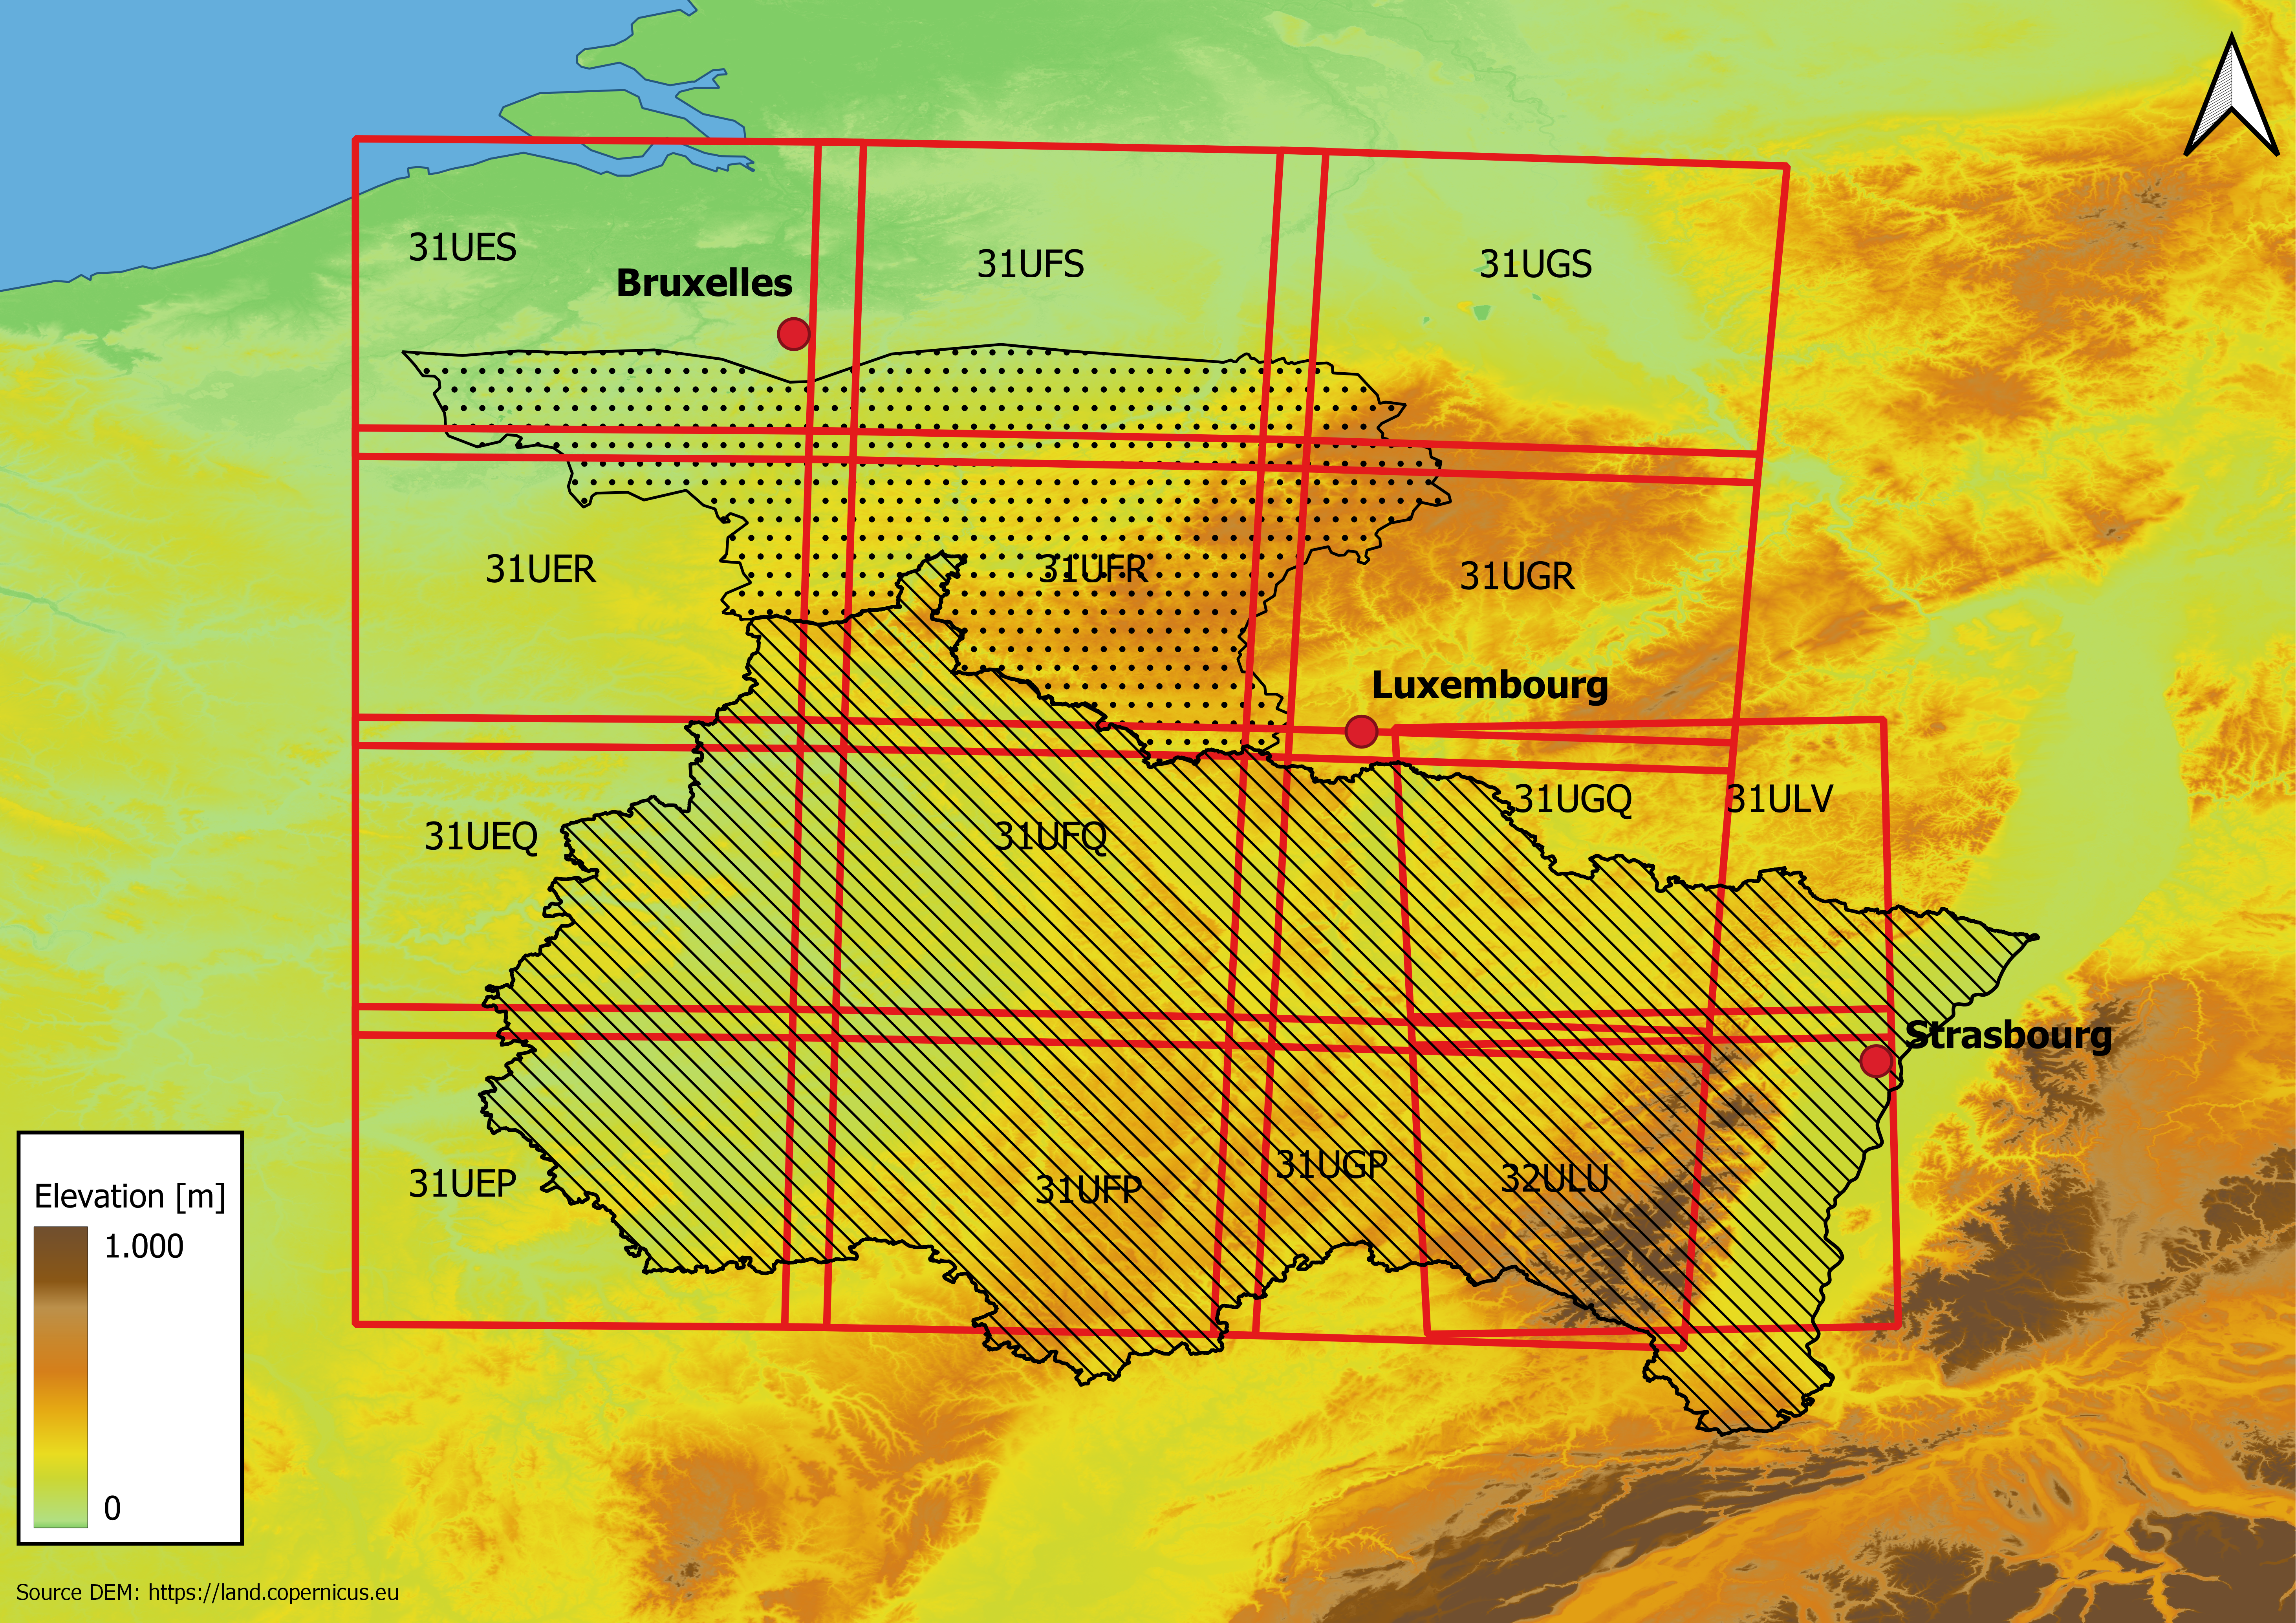
\includegraphics[width=0.7\textwidth]{gde.jpeg}
	\caption{Study area: Grand-est(hashed) and Wallonia (black dot), tile Sentinel 2 (red square)!!!è§}
	\label{fig:situ}
\end{figure}
In Wallonia, the altitude varies between 100 and 700m.
The walloon forest covers 554 600 Ha. 
The norway spruce stand occuped 139 600 Ha \citep{Alderweireld_2015}. 
%For this study, we selected only spruce trees over 15 m and we have worked on 90 500 Ha in Wallonia. 
Two thirds of the Walloon spruce forest is located above 400m altitude. 
The Walloon climate is located in the temperate oceanic bioclimatic zone \citep{lindner_climate_2010}. 
Over the 1989-2020 period, the average temperature vary between 8,7°C and 10,7°C and the average sum of rainfall range from 800m and 1120mm. 
During 2018, the average temperature was 9°C between 11,7°C and the average sum of rainfall varie between 605 mm and 1015 mm (data of Institut Royal Métérologique). 
%The month of july 2018 is considered as a arid month. 
In the Grand-Est, the elevation is between 100m and 1300m. 
The Grand-est forest occupies 1 939 000 ha. 
The norway spruce forest covers 136 000 Ha \citep{IGN2022}. 
%In this study, we worked on 125 800 ha of spruce in this region.
The majority of norway spruce stand of this region grow between 400m and 900m. 
The Grand-est is included in the temperate oceanic bioclimatic zone\citep{lindner_climate_2010}. 
During the 1989-2020 period, the average temperature was between  8,4°C and 11,2°C et the average sum of rainfall range from 720 mm and 1475 mm. During the year 2018, the average temperature vary between 10,16°C and 12,4°C et the average sum of rainfall was 640 mm and 1362mm.
\begin{figure}
	\centering
	\includegraphics[width= 0.8\textwidth]{clim_region_nat_GE_Wal_en.jpg}
	\caption{	}
	
	\label{fig:clim}
\end{figure}
%The 3 primary regions of production of norway spruce in Wallonia are the "Basse et Moyenne Ardenne", "Ardenne centro oriental" and the "Haute ardenne" \citep{van_der_perre_carte_2015}. 
%In the Grand-Est, the major part of the norway spruce stand is located in the 3 naturals regions of the Vosges (Vosges Gréseuses, Vosges cristallines, les collines sous-vosgiennes).
%For the growing season, in this 2 primary regions of production of noraway spruce, there are a lack of 100 mm of water for 2018 and there is a increasing of 1,7 °C compared to 30-year temperatures.(Figure \ref{fig:clim}). 

%Pour la saison de vegetation, les moyennes de températures et des précipitations montre que l'année 2018 fut plus séche et plus chaude que la moyenne trentenaire. 


%\subsection{Description zone de la Zone d'étude}

%\begin{itemize}
%	\item Description zone d'étude générale + tuile S2 traitées (figure: %\ref{fig:rep_vosg}) 
%	\item Description générale de la forêt wallonne 
%	\item Description de la pessière wallonne 
%	\item Description générale de la foret vosgienne 
%	\item Description de la pessière vosgienne
	%\item Comparaison Température et précipitation vosges et Wallonie entre moyenne trentenaire et données pour l'année 2018 (figure reffig:diagOT)
	
%\end{itemize}



\subsection{Description of environmental description}


We have used the digital surface model data from the Copernicus Land Monitoring Service \citep{DEM_copernicus}  at a resolution of 25mX25m for all elevation data and slope calculations.
%European Union, Copernicus Land Monitoring Service <year>, European Environment Agency (EEA)
%\begin{itemize}
%	\item Provenance des données de MNT
%	\item Méthodologie de calcul des sous-secteur radiatif.
%\end{itemize}
Solar orientation influences bark beetle capture in pheromone traps \citep{AFR64}.
We determined this solar orientation using the \cite{Delvaux_galoux} definition of the 3 topography orientations.
%For the three topography orientation (cold slope, plateau, hot slope), we applied the definition of Delvaux and Galoux (1962):
Plateau and low slope are slope less than  20\% that does not create a particular micro-climate. 
Cold slopes are slopes greater than  20\% facing north and valley bottom. 
These are shady, cool and humid areas. 
Warm slopes are slope greater than  20\% facing south. 
In this orientation the air is warmer and drier and the temperature difference between day and night is greater.
Based on this definition and on the DEM, we produced topography orientation  maps for Wallonia and the Grand-Est.
Climate data for Wallonia have been provided by the Institut Royal Météorologique(IRM). The resolution of the data is 5km X 5km. Climate data of  Grand-est come from the data base Digitalis \citep{piedallu_presentation_2014}. The resolution of this data is 1km X 1km.

%MNH

\subsection{Mapping of spruce dieback and mortality by analysis of sentinel-2 time-serie}


The European Union’s earth observation programme, with its satellite twin constellation Sentinel-2A and Sentinel-2B, provides free earth imagery with a high revisit time. 
Sentinel-2 (S2) satellites carry multispectral sensor with a ground resolution up to 10 m. 
S2 imagery have been intensively used recently for forestry purpose, including for the monitoring of bark beetle outbreaks. 
Low and Koukal \citep{low_phenology_2020} have modelled phenology courses of vegetation indices to detect forest disturbances. 
They have properly mapped Bark beetle infestation in Austrian spruce stands.
\cite{ali_canopy_2021} have used multi-years time series remote sensing data in order to detect early bark beetle infestation in Germany. 
They have highlighted the potential of S2 data for the production of reliable infestation maps.
\cite{barta_early_2021} have studied spectral trajectories of nine bands and six vegetation indices from S2 imagery for the 2018 vegetation season. 
They have confirmed the superiority of multi-date data for the classification by Random Forest of infested stands in the Czech Republic.

In this present research, the detection of bark beetle infestation is realized by using dense time series of S2 imagery following the methodology developped by \cite{dutrieux_package_2021}.
The two regions  studied are covered by 14 Sentinel-2 tiles (Figure \ref{fig:situ}).  
Vegetation changes are tracked by means of a phenology metric, the \textit{SWIR Continuum Removal} ($SWIR_{CR}$) indice.
All S2 acquisitions are used in the analyses, provided that the cloud couver do not excess 35 percent. 
Bottom Of Atmosphere reflectance images (L2A product) are downloaded from the Theia data cluster \citep{theia_team} for all the 6 granules, which are tiles of 100km x 100km, that covers Wallonia. 
For north France, 10 granules cover the Grand-Est.
The $SWIR_{CR}$ is based on three spectral bands, the near-infrared, the shortwave infrared 1 band and the shortwave infrared 2, and is sensitive to the foliage water content (figure \ref{fig:harmo}).
Seasonal variation of $SWIR_{CR}$ for healthy stand is modelled and a bark beetle attack is detected if the observations deviates from the healthy phenology trajectory. 
Figure \ref{fig:harmo} illustrates a time-serie of $SWIR_{CR}$ observations (grey dots) for one pixel. 
In 2018, the observations goes beyond the threshold represented by the purple-dashed line, which shows that the spruce stand suffer from a serious stress induced by a bark beetle attack.
A bark beetle outbreak is confirmed as soon as $SWIR_{CR}$ vegetation indice show a stress for at least three consecutive times.
In parallel to the detection of bark beetle stress, stand cutting and thinning are subject of particular attention. 
Bare soil is detected by using a combination of red, green and shortwave infrared reflectance values.
Cutting are thus taken into account and are classified either as normal harvest cutting or as sanitary thinning based on the health status prior to the cutting.
The analysis of image time-serie is thus quite straightforward and is performed individually pixel per pixel starting from the 2016 year, which is the beginning of S2 acquisitions. 
The dense time-serie covers the 2016-2021 period and count a minimum of 180 acquistion dates. 
The health status is summarized in annual health maps by means of four classes ; healthy, bark beetle attached, cutted and sanitary thinning.

\begin{figure}
	\centering
	\includegraphics[width=0.8\textwidth]{fctHarmo.png}
	\caption{Bark beetle infestation map are computed by detecting change in the $SWIR_{CR}$ phenology metric. The \textit{SWIR Continuum Removal} is computed using three bands from Sentinel-2 imagery for every single acquisition date and his value is compared to a threshold (purple dashed line) in order to detect vegetation stress. If a stress is detected three consecutive times, we assume that a bark beetle infection occured.}
	\label{fig:harmo}
\end{figure}

Our approach of bark beetle detection is only suitable for spruce, as it is closely related to the phenological course of healthy spruce forest.
An essential prerequisite is thus to have a proper mapping of spruce stands.
For the south of Belgium, we use existing reliable composition maps \citep{bolyn_forest_2018} computed from remote sensing data in order to restrict our analysis to spruces.

In the Grand-est, the composition map comes from the French Mapping agency (Forest BD version 2). 
Composition of forest stand is determined by photointerpretation and forest stands identifyed as "spruce or fir" serve as starting point to limit our analysis.
Time series are a convenient means to track phenology changes. 
More broadly than the dectection of bark beetle infestion, phenology courses are highly suitable for forest tree species discrimination \citep{lisein_discrimination_2015,grabska_forest_2019,ma_tree_2021}.
We have used S2 spectral bands courses along the vegetation season to refine the determination of species present in the area interpreted as "spruce or fir" in Vosges.
The objective is to identify and remove every area that are not spruce stand, as pixels located on others species than spruce are likely to be wrongly detected as a bark beetle attack.
All S2 spectral bands were first summarized for each of the four trimesters of the year, by simply averaging all observations occuring during the trimester.
Then, a Random Forest algorithm was trained on these synthetic intra-annual time serie to discriminate spruce from non-spruce pixels, based on a training set of observation from Belgium \citep{bolyn_forest_2018}.
Eventually, this Random Forest classifier was applied on "spruce and fir" area of Vosges and bark beetle detection was carried on only for pixels detected as spruce. 


%modif vosges by grand est



\subsection{Relation between bark beetle attack and environmental condition}

\subsubsection{Choice of important variables}

We try to choice the two most important environmental variable that influence the attack of bark beetle.
We make a resample spruce mask in tile of 50mX50m (the minimum area to make productive silviculture). Each tile corresponds to a productive stand. 
We extract for all of stand the value of environmental variables.  
To select the important variables influenced the attack of bark beetle, the random forest algorithm is used \citep{genuer_vsurf_2015}.
Individual classification trees are trained on a 1000 samples of spruce stand of 0,25 Ha by randomly selecting a subset of explanatory variables.




\subsubsection{Variation of attack along important gradient}
For this study, we selected only spruce trees over 15 m and we have worked on 90 500 Ha in Wallonia and  on 125 800 ha of spruce in the Grand-est region.  
			
% Classe d'latitude
%calcul prob prese
%Comparaison entre le différents pays
%Depuis 2018, des attaques massives de scolytes tuant les épicéas frappent la Wallonie. Suite à ces évenements,les forestiers se sont interrogés sur cerains facteurs topographiques semblant avoir fortement influencé les attaques de scolytes.
%Les pessières situées en basse altitude semblent avoir été plus touché ainsi que les peuplement situé sur des versants sud.

%Pour caracteriser les attaques de scolytes, nous avons appliquer la méthode des random forest afin de selectionner les 2 facteurs topographiques influençant le plus les attaques de scolytes. CEs deux facteur sont l'altitude et les sous-radiatif. Nous avons ventilé l'altitude par classe de 100m et conservé les trois classes de sous secteurs définis par delvaux et galoux.

%Ensuite, afin de determiner les classes de ces facteurs les plus impactés par le scolyte, nous avons estimé les surfaces scolytés pour chacune des classes de chaque facteurs sur base des cartes d'état sanitaire pour chaque année de la période 2016-2021.

%La carte d'etat sanitaire de la pessière a été subdivisée en tuile de 50*50m (25 pixel de 10X10m) comprenant au minimum 17 pixel de 10mX10m d'épicéas. Une tuile est considérée comme %scolytée quand minimum 3 pixels sur 25 sont scolytés.

%Pour chaque tuile, la classe d'altitude et le sous-secteur ont été extraits.

%Nous avons calculé le ratio du nombre tuiles scolyté d'une classe divisé par le nombre total de tuiles de la classe (probabilité de présence) pour chacune des classes d'altitude et de sous-secteurs.


%\begin{align*}

%$presence\,of\,probability = \frac{tiles\, affected\, by\, the\, bark\, beetle\, of\, a\, class}{total\, number\, of\, tiles\, in\, the\, class}$

%\end{align*}


Since 2018, massive bark beetle attacks killing spruce trees have been occurring in Wallonia and in the Grand-Est. Following these events, foresters have asked themselves about certain topographical factors that seem to have strongly influenced bark beetle attacks. 
The spruce forests located at low altitude seem to have been more affected as well as the stands located on southern slopes.
%However, other factors such as degres day data could influence bark beetle attacks 
%We made a selection of factors influencing bark beetles favourably and norway spruce unfavourably using the random forest method. The factors emerging from this analysis show that altitude and radiative topography orientation are the most important factors influencing spruce dieback  
To characterise the bark beetle attacks, we applied the random forest method to select the two topographic factors that most influenced the bark beetle attacks.
These two factors are altitude and topography orientation. We broke down the altitude by 100m classes and kept the three topography orientations classes defined by \cite{Delvaux_galoux}.
Then, in order to determine the classes of these factors most impacted by the bark beetle, we estimated the bark beetle areas for each class of each factor based on the sanitary status maps for each year of the period 2016-2021.

%The spruce health map was subdivided into 50*50m tiles (25 pixels of 10X10m) comprising at least 17 pixels of 10mX10m spruce. A tile is considered to be barked when at least 3 out of 25 pixels are barked.For each tile, elevation class, topography orientation and the sanitary status were extracted. We calculated the ratio of the number of tiles attacked by bark beetle in a class divided by the total number of tiles in the class (probability of occurrence) for each of the elevation and topography orientation classes.




%\begin{itemize}
%	\item Random forest  
	

%	\item test de student
%	\item the probability of presence of bark beetles
%The probability of bark beetle presence is the area affected by bark beetle attacks on the total spruce area. 



%Equation 
%\end{itemize}


\section{Results}

\subsection{Choice of environmental variable}




\subsection{ Elevation vs bark beetle presence}
The variation of the probability of presence of bark beetles for Wallonia and Grand-Est for the period 2017-2021 is described in the figure 
\ref{alti_sco}.
%The altitude has been subdivided into the same 12 elevation classes for both regions. 
%The graphs corresponding to the variation of the probability of presence in Wallonia are in the upper part of the figure and those for the Grand-Est in the lower part.

\begin{figure}
\centering
	\includegraphics[width=\textwidth]{graphe_wall_GDE.png}
     \caption{The altitude has been subdivided into the same 12 elevation classes for both regions. 
The graphs corresponding to the variation of the probability of presence in Wallonia are in the upper part of the figure and those for the Grand-Est in the lower part.
}
	\label{alti_sco}
\end{figure}

In Wallonia, in the begin of the crisis, the low altitude classes are more affect than hight altitude classes.
The dieback of norway spruce occur along a altitudinal  gradient.
This gradient is confirmed over the 5 years of the study.
%Indeed, during this year a strong increase in the 100-200m and 200-300m altitude classes is observed. 
%These two altitude classes are more affected during this crisis.
The low altitude stand are the more affected stand and are disappearing.
 
%The decrease the probabilty of bark beetle presence follow an altitudinal gradient.
%The higher the norway spruce stand grows at an altitude, the lower the probabilty of bark beetle presence. 
%For the Grand-Est region, there is an increase in the probability of bark beetle presence between 2019 and 2021. 

In the Grand-Est stand, the situation differs than is neighbour region. In 2017, there is low presence of bark beetle  at all altitude.
The crisis begin weakly in 2018 with attack at low altitude.
However the probability of presence of bark beetle increase until 2020 to reach more than 20\% of norway spruce killed at altitude below 300m.
Above 400m, the decreasing didn't follow a altitudinal gradient.
The probability of presence of bark beetle is relatively constant with a little increase between 700-800m.
Above 400m, the altitude didn't protect spruce against bark beetle attack in the Grand-Est.

%Unlike the Walloon spruce forest, there is no clear altitudinal gradient in the Vosges. 
%As in Wallonia, the 200-300m altitude class is strongly affected by the bark beetle. The probability of presence decreases along an altitudinal gradient between the altitude classes 200-300 and 400-500m. However, above 500m the probability of bark beetle increases up to the altitude class 700-800m.
%_Description figure \ref{fig:sco_alti} 
% augmentation de la probabilité de présence jusqu'en 2020 et diminution en 2021
% Wallonie: Diminution de la probabilité de présence de scolyte avec l'augmentation de l'altitude 
% Vosges pas de relation clair avec l'altitude. Cependant, les classes d'altitude 2, 11 et 12 semblent + touchées que les autres classes d'altitude
% et ne pas oubnlier de citer untel et machin
	
% Wallonie + Vosges: Augmentation de la probabilité de présence de scolyte avec le temps quelque soit la classe d'altitude.


\subsection{topography orientation vs bark beetle presence}

%Le scolyte se develloppant plus rapidement dans les zones plus chaudes \citep{annila_influence_1969}, nous %avons étudié l'évolution de la surface d'épicéa imapactée par les scolytes en fonction des sous-secteur %radiatif.

% Le pic de surface touchée par les scolytes est atteint en 2019 pour la Wallonie et en 2020 pour le Grand-Est.
%Ce graphe montre aussi que proportionelemnt parlant les pessières des plaines du grand-est ont été plus touchée que les autres sous-secteurs aussi bien du grand-est que de Wallonie.
 
% En Wallonie, les sous secteurs les plus touchés significativement sont les versants.On observe aussi une différence significative entre versant sud et nord. 
 
%A l'inverse, dans le grand-est ce sont les plateaux qui sont significativement plus touchés que les versants.


% As the bark beetle develops more rapidly in warmer areas \citep{annila_influence_1969}, we studied the evolution of the surface area of spruce affected by bark beetles as a function of the topography orientation.
The second environmental factor emerging from our analysis is topography orientation. 
The peak of bark beetle affected area is reached in 2019 for Wallonia and in 2020 for the Grand-Est (Figure \ref{ss_sco}).
This graph also shows that proportionally the spruce forests of the plains of the Great East were more affected than the other topography orientation in both the Grand-Est and Wallonia. 
In Wallonia, the most significantly affected topography orientation are the slopes, and there is also a significant difference between the southern and northern slopes. 
Conversely, in the Grand Est it is the plateaus that are significantly more affected than the slopes.
\begin{figure}
\centering
	\includegraphics[width=\textwidth]{evol_ss_GDE_wall.png}
     \caption{Proportion area affected by bark beetle attacks in relation to topography orientation. Dotted line: Wallonia , line : Grand-Est }
	\label{ss_sco}
\end{figure}

%\begin{itemize}
%	\item Description figure \ref{fig:ss_wall} 
%	\item Wallonie: Différences significative entre les différents sous secteurs. Les sous secteur froid sont  plus touchés que les sous secteur chaud et les plateaux. Les plateaux sont moins touché en Wallonie.
%	\item Vosges: pas de différence significative entre les sous secteurs ( \ref{fig:ss_vosg})
	
%\end{itemize}

%sous-secteur
%graphe + descruipton


\subsection{Evolution et importance}

The evolution of the crisis differs between these two neighbouring regions. 
In Wallonia, during the year 2017 and 2018, there are already norway spruce affected by bark beetle in low elevation but the probability of presence is under 10\%. 
In 2019, the peak is reached in all of classe of elevation. During this year, the percentage of area of the Wallon norway spruce stand affected by bark beetle is 2.8\%.
In 2020, there a  little diminution of attack. 
During 2021, there are important diminution of area impacted by bark beetle. The probability of bark beetle presence returns to the same level as begin the crisis.

In Grand-Est, during 2017, the attack of bark beetle are weak. 
In 2018, there are first attack at low elevation but always below 5\%.
In 2019, the increasing of attack at low altitude continues.
In 2020, in all altitude classes are impacted by bark beetle. 
Between 100m an 400m of altitude there are a important augmentation of the probability of presence. 
The maximum of area affected is reached. % indiqué pourcentage max atteint
During 2020, there is 4\% of the total area of spruce stand of Grand-est that area affected by bark beetle during 2020.

 
  




\section{Discussion}

\subsection{Différence entre Vosges et Wallonie}
\begin{itemize}
	\item Différence climat (Climat semicontinental/montagnard vs climat tempéré océanique)
	\item Différence sylvicole ( Wallonie futaie régulière exploitable vs Vosges peuplement + mélangé et moins exploitable en haute altitude)
	\item Sommet des vosges epicéas endémiques vs épicéas en plantations (résilience peuplement )
	\item adaptation ep à condition plus rude en versant sud que nord 
	D'après la theorie il devrait y avoir plus de generation sur versant sud car car + chaud et donc pluys touché
	Seuil letal ou the letargie atteint en versant sud?
\item meilleur surveillance des forestiers sur versant sud que nord 
	
\end{itemize}

\subsection{Facteur déterminant l'attaque par l'épicéa ou le scolyte}

\begin{itemize}
	\item Discussion généralisation de modèle scolyte/ dépérissement des épicéas
    \item est ce la Biologie du scolyte/ ou le stress de l'épicéa qui conditionne le dépérissement massif ?
	
\end{itemize}

\section{Conclusion}

%Dans des régions très proches, les stations de dépérissement de l'épicéa sont différentes.
%Il semble donc difficle de généraliser des modèles basé sur des relations topographique à une grande échelle. 
\section{Figure}


	

%\begin{figure}[htbp]
%	\begin{minipage}[b]{1 \linewidth}
%		\centering
	%	\includegraphics[width=1\textwidth]{evol_ss_wal.png}
%		\caption{Évolution de la crise du typographe en région wallonne en fonction des sous-secteurs.}
%		\label{fig:ss_wall}
		%\caption sert à insérer une légende
%	\end{minipage}\hfill
%	\vspace{1cm}
%	\begin{minipage}[b]{1 \linewidth}
%		\centering
%		\includegraphics[width=1\textwidth]{evol_ss_vosges.png}
%		\caption{Évolution de la crise du typographe dans les Vosges en fonction des sous-secteurs .}
%		\label{fig:ss_vosg}
%	\end{minipage}
%end{figure}

\section{Acknowledgements}

This research has been funded thanks to the \textit{RegioWood II} project.

%\bibliographystyle{elsarticle-num}
\bibliographystyle{plainnatGL_v2}\biboptions{authoryear}
\bibliography{Scolyte.bib}
\end{document}